\documentclass[twoside]{book}

% Packages required by doxygen
\usepackage{fixltx2e}
\usepackage{calc}
\usepackage{doxygen}
\usepackage{graphicx}
\usepackage[utf8]{inputenc}
\usepackage{makeidx}
\usepackage{multicol}
\usepackage{multirow}
\PassOptionsToPackage{warn}{textcomp}
\usepackage{textcomp}
\usepackage[nointegrals]{wasysym}
\usepackage[table]{xcolor}

% Font selection
\usepackage[T1]{fontenc}
\usepackage{mathptmx}
\usepackage[scaled=.90]{helvet}
\usepackage{courier}
\usepackage{amssymb}
\usepackage{sectsty}
\renewcommand{\familydefault}{\sfdefault}
\allsectionsfont{%
  \fontseries{bc}\selectfont%
  \color{darkgray}%
}
\renewcommand{\DoxyLabelFont}{%
  \fontseries{bc}\selectfont%
  \color{darkgray}%
}
\newcommand{\+}{\discretionary{\mbox{\scriptsize$\hookleftarrow$}}{}{}}

% Page & text layout
\usepackage{geometry}
\geometry{%
  a4paper,%
  top=2.5cm,%
  bottom=2.5cm,%
  left=2.5cm,%
  right=2.5cm%
}
\tolerance=750
\hfuzz=15pt
\hbadness=750
\setlength{\emergencystretch}{15pt}
\setlength{\parindent}{0cm}
\setlength{\parskip}{0.2cm}
\makeatletter
\renewcommand{\paragraph}{%
  \@startsection{paragraph}{4}{0ex}{-1.0ex}{1.0ex}{%
    \normalfont\normalsize\bfseries\SS@parafont%
  }%
}
\renewcommand{\subparagraph}{%
  \@startsection{subparagraph}{5}{0ex}{-1.0ex}{1.0ex}{%
    \normalfont\normalsize\bfseries\SS@subparafont%
  }%
}
\makeatother

% Headers & footers
\usepackage{fancyhdr}
\pagestyle{fancyplain}
\fancyhead[LE]{\fancyplain{}{\bfseries\thepage}}
\fancyhead[CE]{\fancyplain{}{}}
\fancyhead[RE]{\fancyplain{}{\bfseries\leftmark}}
\fancyhead[LO]{\fancyplain{}{\bfseries\rightmark}}
\fancyhead[CO]{\fancyplain{}{}}
\fancyhead[RO]{\fancyplain{}{\bfseries\thepage}}
\fancyfoot[LE]{\fancyplain{}{}}
\fancyfoot[CE]{\fancyplain{}{}}
\fancyfoot[RE]{\fancyplain{}{\bfseries\scriptsize Generated on Thu May 11 2017 13\+:29\+:30 for chifoumi by Doxygen }}
\fancyfoot[LO]{\fancyplain{}{\bfseries\scriptsize Generated on Thu May 11 2017 13\+:29\+:30 for chifoumi by Doxygen }}
\fancyfoot[CO]{\fancyplain{}{}}
\fancyfoot[RO]{\fancyplain{}{}}
\renewcommand{\footrulewidth}{0.4pt}
\renewcommand{\chaptermark}[1]{%
  \markboth{#1}{}%
}
\renewcommand{\sectionmark}[1]{%
  \markright{\thesection\ #1}%
}

% Indices & bibliography
\usepackage{natbib}
\usepackage[titles]{tocloft}
\setcounter{tocdepth}{3}
\setcounter{secnumdepth}{5}
\makeindex

% Hyperlinks (required, but should be loaded last)
\usepackage{ifpdf}
\ifpdf
  \usepackage[pdftex,pagebackref=true]{hyperref}
\else
  \usepackage[ps2pdf,pagebackref=true]{hyperref}
\fi
\hypersetup{%
  colorlinks=true,%
  linkcolor=blue,%
  citecolor=blue,%
  unicode%
}

% Custom commands
\newcommand{\clearemptydoublepage}{%
  \newpage{\pagestyle{empty}\cleardoublepage}%
}


%===== C O N T E N T S =====

\begin{document}

% Titlepage & ToC
\hypersetup{pageanchor=false,
             bookmarks=true,
             bookmarksnumbered=true,
             pdfencoding=unicode
            }
\pagenumbering{roman}
\begin{titlepage}
\vspace*{7cm}
\begin{center}%
{\Large chifoumi }\\
\vspace*{1cm}
{\large Generated by Doxygen 1.8.8}\\
\vspace*{0.5cm}
{\small Thu May 11 2017 13:29:30}\\
\end{center}
\end{titlepage}
\clearemptydoublepage
\tableofcontents
\clearemptydoublepage
\pagenumbering{arabic}
\hypersetup{pageanchor=true}

%--- Begin generated contents ---
\chapter{Chifoumi\+\_\+\+G\+L}
\label{index}\hypertarget{index}{}\hypertarget{index_intro_sec}{}\section{Chifoumi}\label{index_intro_sec}
Realisation d'un chifoumi en c++, respectivement en version \char`\"{}terminal\char`\"{} et en interface graphique. Chifoumi utilise les bibliothèque ccputest et libglog pour les test unitaires et les logs. 
\chapter{File Index}
\section{File List}
Here is a list of all files with brief descriptions\+:\begin{DoxyCompactList}
\item\contentsline{section}{/etudiants/qcoloos/\+Documents/\+G\+L/\+L3\+\_\+\+G\+L\+\_\+etudiant/\+Projet\+\_\+chifoumi/src/\hyperlink{chifoumi_8cpp}{chifoumi.\+cpp} }{\pageref{chifoumi_8cpp}}{}
\item\contentsline{section}{/etudiants/qcoloos/\+Documents/\+G\+L/\+L3\+\_\+\+G\+L\+\_\+etudiant/\+Projet\+\_\+chifoumi/src/\hyperlink{main__test_8cpp}{main\+\_\+test.\+cpp} }{\pageref{main__test_8cpp}}{}
\end{DoxyCompactList}

\chapter{File Documentation}
\hypertarget{chifoumi_8cpp}{\section{/etudiants/qcoloos/\+Documents/\+G\+L/\+L3\+\_\+\+G\+L\+\_\+etudiant/\+Projet\+\_\+chifoumi/src/chifoumi.cpp File Reference}
\label{chifoumi_8cpp}\index{/etudiants/qcoloos/\+Documents/\+G\+L/\+L3\+\_\+\+G\+L\+\_\+etudiant/\+Projet\+\_\+chifoumi/src/chifoumi.\+cpp@{/etudiants/qcoloos/\+Documents/\+G\+L/\+L3\+\_\+\+G\+L\+\_\+etudiant/\+Projet\+\_\+chifoumi/src/chifoumi.\+cpp}}
}
{\ttfamily \#include $<$iostream$>$}\\*
{\ttfamily \#include $<$glog/logging.\+h$>$}\\*
Include dependency graph for chifoumi.\+cpp\+:\nopagebreak
\begin{figure}[H]
\begin{center}
\leavevmode
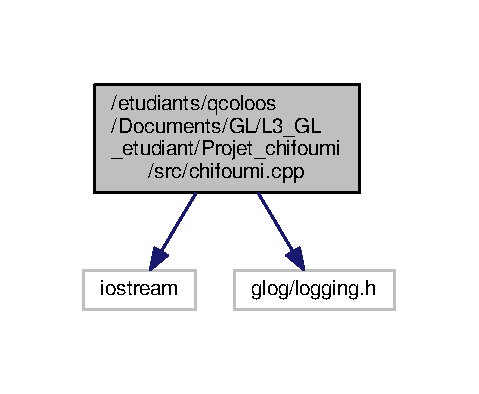
\includegraphics[width=230pt]{chifoumi_8cpp__incl}
\end{center}
\end{figure}
\subsection*{Functions}
\begin{DoxyCompactItemize}
\item 
int \hyperlink{chifoumi_8cpp_a3c04138a5bfe5d72780bb7e82a18e627}{main} (int argc, char $\ast$$\ast$argv)
\end{DoxyCompactItemize}


\subsection{Function Documentation}
\hypertarget{chifoumi_8cpp_a3c04138a5bfe5d72780bb7e82a18e627}{\index{chifoumi.\+cpp@{chifoumi.\+cpp}!main@{main}}
\index{main@{main}!chifoumi.\+cpp@{chifoumi.\+cpp}}
\subsubsection[{main}]{\setlength{\rightskip}{0pt plus 5cm}int main (
\begin{DoxyParamCaption}
\item[{int}]{argc, }
\item[{char $\ast$$\ast$}]{argv}
\end{DoxyParamCaption}
)}}\label{chifoumi_8cpp_a3c04138a5bfe5d72780bb7e82a18e627}

\hypertarget{main__test_8cpp}{\section{/etudiants/qcoloos/\+Documents/\+G\+L/\+L3\+\_\+\+G\+L\+\_\+etudiant/\+Projet\+\_\+chifoumi/src/main\+\_\+test.cpp File Reference}
\label{main__test_8cpp}\index{/etudiants/qcoloos/\+Documents/\+G\+L/\+L3\+\_\+\+G\+L\+\_\+etudiant/\+Projet\+\_\+chifoumi/src/main\+\_\+test.\+cpp@{/etudiants/qcoloos/\+Documents/\+G\+L/\+L3\+\_\+\+G\+L\+\_\+etudiant/\+Projet\+\_\+chifoumi/src/main\+\_\+test.\+cpp}}
}
{\ttfamily \#include $<$Cpp\+U\+Test/\+Command\+Line\+Test\+Runner.\+h$>$}\\*
Include dependency graph for main\+\_\+test.\+cpp\+:\nopagebreak
\begin{figure}[H]
\begin{center}
\leavevmode
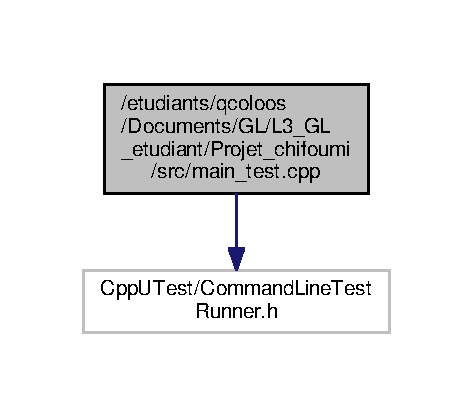
\includegraphics[width=227pt]{main__test_8cpp__incl}
\end{center}
\end{figure}
\subsection*{Functions}
\begin{DoxyCompactItemize}
\item 
int \hyperlink{main__test_8cpp_a3c04138a5bfe5d72780bb7e82a18e627}{main} (int argc, char $\ast$$\ast$argv)
\end{DoxyCompactItemize}


\subsection{Function Documentation}
\hypertarget{main__test_8cpp_a3c04138a5bfe5d72780bb7e82a18e627}{\index{main\+\_\+test.\+cpp@{main\+\_\+test.\+cpp}!main@{main}}
\index{main@{main}!main\+\_\+test.\+cpp@{main\+\_\+test.\+cpp}}
\subsubsection[{main}]{\setlength{\rightskip}{0pt plus 5cm}int main (
\begin{DoxyParamCaption}
\item[{int}]{argc, }
\item[{char $\ast$$\ast$}]{argv}
\end{DoxyParamCaption}
)}}\label{main__test_8cpp_a3c04138a5bfe5d72780bb7e82a18e627}

%--- End generated contents ---

% Index
\newpage
\phantomsection
\addcontentsline{toc}{chapter}{Index}
\printindex

\end{document}
